%%%%%%%%%%%%%%%%%%%%%%%%%%%%%%%%%%%%%%%%%%%%%%%%%%%%%%%%%%%%%%%%%%%%%%
\NeedsTeXFormat{LaTeX2e}
\documentclass[12pt,a4paper]{article}

%-- used packages ------------------------------------------------------

\usepackage{amsmath}
\usepackage{amssymb}
\usepackage{epsfig}
\usepackage{graphicx}
\usepackage{cite}
%\usepackage{mcite}
%-- page parameters -------------------------------------------------

\jot = 1.5ex
\parskip 5pt plus 1pt
\parindent 0pt
\evensidemargin -0.1in   \oddsidemargin  -0.1in
\textwidth  6.45in       \textheight 9.1in
\topmargin -1.0cm        \headsep    1.0cm

%-- command (re)definitions -----------------------------------------


\newcommand{\capdef}{}
%\newcommand{\mycaption}[2][\capdef]{\renewcommand{\capdef}{#2}%
%       \caption[#1]{{\itshape #2}}}
\newcommand{\mycaption}[2][\capdef]{\renewcommand{\capdef}{#2}%
       \caption[#1]{{\footnotesize #2}}}
\makeatletter
\renewcommand{\fnum@table}{\textbf{\tablename~\thetable}}
\renewcommand{\fnum@figure}{\textbf{\figurename~\thefigure}}
\makeatother
\def\ltap{\ \raisebox{-.4ex}{\rlap{$\sim$}} \raisebox{.4ex}{$<$}\ }
\def\gtap{\ \raisebox{-.4ex}{\rlap{$\sim$}} \raisebox{.4ex}{$>$}\ }

\newcounter{myenumi}
\newcommand{\myitem}{\refstepcounter{myenumi}\item}
\renewcommand{\themyenumi}{\roman{myenumi}}
\newenvironment{mylist}{%
        \setcounter{myenumi}{0}
        \begin{list}{\textit{\themyenumi)}}{%
        \setlength{\topsep}{0.2\baselineskip}%
        \setlength{\partopsep}{-\topsep}%
        \setlength{\itemsep}{\topsep}%
        \setlength{\parsep}{0\baselineskip}%
        \setlength{\leftmargin}{0em}%
        \setlength{\listparindent}{\parindent}%
        \setlength{\itemindent}{2.5em}%
        \setlength{\labelwidth}{1.5em}%
        \setlength{\labelsep}{0.75em}}}%
{\end{list}}

\newlength{\myem}
\settowidth{\myem}{m}
\newcommand{\sep}[1]{#1}
\newcounter{mysubequation}[equation]
\renewcommand{\themysubequation}{\alph{mysubequation}}
\newcommand{\mytag}{\stepcounter{mysubequation}%
\tag{\theequation\protect\sep{\themysubequation}}}
\newcommand{\globallabel}[1]{\refstepcounter{equation}\label{#1}}

\makeatletter
\renewcommand{\section}{\@startsection{section}{1}{0em}{-\baselineskip}%
{\baselineskip}{\normalfont\large\bfseries}}
\renewcommand{\subsection}%
{\@startsection{subsection}{2}{0em}{-0.7\baselineskip}%
{0.7\baselineskip}{\normalfont\bfseries}}
\makeatother

\newcommand{\ie}{{\it i.e.}}
\newcommand{\Ie}{{\it I.e.}}
\newcommand{\eg}{{\it e.g.}}
\newcommand{\Eg}{{\it E.g.}}
\newcommand{\cf}{{\it cf.}}
\newcommand{\etc}{{\it etc.}}
\newcommand{\eq}{Eq.}
\newcommand{\eqs}{Eqs.}
\newcommand{\Def}{Definition}
\newcommand{\fig}{Fig.}
\newcommand{\Fig}{Fig.}
\newcommand{\figs}{Figs.}
\newcommand{\Figs}{Figs.}
\newcommand{\Ref}{Ref.}
\newcommand{\Refs}{Refs.}
\newcommand{\Sec}{Sec.}
\newcommand{\Secs}{Secs.}
\newcommand{\Chapt}{Chapter}
\newcommand{\Chapts}{Chapters}
\newcommand{\Part}{Part}
\newcommand{\App}{Appendix}
\newcommand{\Apps}{Appendices}
\newcommand{\Tab}{Table}
\newcommand{\Tabs}{Tables}

\newcommand{\bi}{\begin{itemize}}
\newcommand{\ei}{\end{itemize}}
\newcommand{\ra}{$\rightarrow$}
\newcommand{\be}{\begin{equation}}
\newcommand{\ee}{\end{equation}}
\newcommand{\bea}{\begin{eqnarray}}
\newcommand{\eea}{\end{eqnarray}}
\newcommand{\nn}{\nonumber}
\newcommand{\ldm}{\Delta m_{31}^2}
\newcommand{\sdm}{\Delta m_{21}^2}
\newcommand{\deltacp}{\delta_{\mathrm{CP}}}
\newcommand{\stheta}{\sin^2 2 \theta_{13}}

\newcommand{\MINOS}{{\sf MINOS}}
\newcommand{\ICARUS}{{\sf ICARUS}}
\newcommand{\OPERA}{{\sf OPERA}}
\newcommand{\JHFSK}{{\sf JHF-SK}}
\newcommand{\NUMI }{{\sf NuMI}}
\newcommand{\ReactorI}{{\sf Reactor-I}}
\newcommand{\ReactorII}{{\sf Reactor-II}}
\newcommand{\JHFHK}{{\sf JHF-HK}}
\newcommand{\NuFactI}{{\sf NuFact-I}}
\newcommand{\NuFactII}{{\sf NuFact-II}}

\newcommand{\GLOBES}{{\sf GLoBES}}
\newcommand{\AEDL}{{\sf AEDL}}
\newcommand{\EDM}{{\sf EDM}}

\newcommand{\equ}[1]{\eq~(\ref{equ:#1})}
\newcommand{\figu}[1]{\fig~\ref{fig:#1}}
\newcommand{\tabl}[1]{\Tab~\ref{tab:#1}}
\newcommand{\tb}{\hspace*{3ex}}

\begin{document}
%%%%%%%%%%%%%%%%%%%%%%%%%%%%%%%%%%%%%%%%%%%%%%%%%%%%%%%%%%%%%%%%%%%%%
%%%%                     Title-page                              %%%%
%%%%%%%%%%%%%%%%%%%%%%%%%%%%%%%%%%%%%%%%%%%%%%%%%%%%%%%%%%%%%%%%%%%%%

\begin{titlepage}

% the footnote symbols are only redefined for the title page !
\renewcommand{\thefootnote}{\alph{footnote}}

\vspace*{-3.cm}
\begin{flushright}
TUM-HEP-YYY/0X\\
%hep-ph/
\end{flushright}

\vspace*{0.5cm}

\renewcommand{\thefootnote}{\fnsymbol{footnote}}
\setcounter{footnote}{-1}

{\begin{center}
{\Large\bf New features in the simulation of neutrino oscillation experiments with GLoBES 3.0}
\end{center}}
{\begin{center}
{\large\bf (General Long Baseline Experiment Simulator)}
\end{center}}
\renewcommand{\thefootnote}{\alph{footnote}}

\vspace*{.8cm}
%\vspace*{.3cm}
{\begin{center} {\large{\sc
                Patrick~Huber\footnotemark[1],~
                Joachim~Kopp\footnotemark[2],~
                Manfred~Lindner\footnotemark[2], \\
                Mark~Rolinec\footnotemark[3],~
                Walter~Winter\footnotemark[4]
                }}

\footnote{All correspondence should be addressed to {\tt globes@mpi-hd.mpg.de}}

\end{center}}
\vspace*{0cm}
{\it
\begin{center}

\footnotemark[1]%${}^,$\footnotemark[2]%
       Department of Physics, University of Wisconsin, \\
       1150 University Avenue, Madison, WI 53706, USA

\vspace*{1mm}

\footnotemark[2]%
       Max--Planck--Institut f\"ur Kernphysik,  \\
       Postfach 10~39~80, D--69029 Heidelberg, Germany 

\vspace*{1mm}

\footnotemark[3]%
       Physik--Department, Technische Universit\"at M\"unchen, \\
       James--Franck--Strasse, 85748 Garching, Germany

\vspace*{1mm}

\footnotemark[4]%
       Universit\"at W\"urzburg, 
       Institut f\"ur theoretische Physik und Astrophysik, \\
       Am Hubland, D-97074 W\"urzburg, Germany

\end{center}}

\vspace*{1cm}


\begin{abstract}
We present Version 3.0 of the GLoBES (``General Long Baseline Experiment Simulator'') software, which is
a simulation tool for short- and long-baseline neutrino oscillation experiments. As new features, \GLOBES\ 3.0 allows the simulation of experiments with multiple detectors by the concept of user-defined systematics.
In addition, the combination with external information, such as from different experiment classes, is 
simplified by the concept of user-defined priors. As far as the probability calculation is concerned, \GLOBES\ 
now provides an interface for the inclusion of non-standard physics without re-compliation of the software. 
The set of experiment descriptions coming with \GLOBES\ has been updated. For example, built-in fluxes are now
provided for the simulation of beta beams.
\end{abstract}


\vspace*{.5cm}


\end{titlepage}

\newpage

\renewcommand{\thefootnote}{\arabic{footnote}}
\setcounter{footnote}{0}

\section{Introduction}

Neutrino oscillations are now established as the leading flavor
transition mechanism for neutrinos in a long history of many experiments, see
\eg , \Ref~\cite{Barger:2003qi}. Future facilities, using accelerator-based
 neutrino beams or a nuclear reactors as neutrino sources, are proposed
for precision measurements of the neutrino oscillation parameters. In the
simulation of these experiments, 
the presence of multiple solutions which are intrinsic to
 neutrino oscillation probabilities~\cite{Fogli:1996pv,Burguet-Castell:2001ez,Minakata:2001qm,Barger:2001yr} 
affect the performance.
Thus optimization strategies are required which maximally exploit 
complementarity between experiments. The \GLOBES\ software package~\cite{Huber:2004ka}
is a  modern experiment  simulation  and analysis tool for
a highly accurate beam and detector simulation. In addition, it provides powerful 
means to analyze correlations and degeneracies, especially for the combination
of several experiments. Compared to a Monte Carlo simulation, which yields a different
result in each run, it simulates the performance of the {\em average} experiment
(see \Ref~\cite{Schwetz:2006md} for a discussion of the meaning of ``average'').
The advantage of such an average prediction is a tremendous performance gain,
which can be used for systematical parameter space scans. In addition, it 
simplified the direct comparison of experiments.

The \GLOBES\ software has, in the past, been used for many studies, some of them
are referred to in the paper. However, recent developments have indicated that extensions
and improvements are necessary. In this work, we present the most important new
features and changes in \GLOBES\ 3.0. For experimentalists, \GLOBES\ now allows
for the implementation of arbitrary systematics, which can also be used for
the simulation of multi-detector experiments. In addition, several extensions
have been included in \AEDL\ (``Abstract Experiment Description Language''), such as
built-in beta beam fluxes and the possibility to use lists as variables.
For phenomenologists, user-defined
priors provide a flexible interface to include external information, such as from
different experiments. In addition, \GLOBES\ now can be used for the simulation
of non-standard physics without re-compiling the \GLOBES\ software.

\section{Concept of \GLOBES }

\GLOBES\ (``General Long Baseline Experiment Simulator'') is a flexible
software tool to simulate and analyze neutrino oscillation 
short- and long-baseline experiments using a 
complete three-flavor description. On the
one hand, it contains a comprehensive abstract experiment definition
language (\AEDL ), which allows to describe 
most classes of long baseline and reactor experiments
at an abstract level. On the other hand, it provides a C-library to 
process the experiment information in order to obtain oscillation
probabilities, rate vectors, and $\Delta \chi^2$-values (\cf, \figu{GLOBES}). 
In addition, it provides a binary program to test experiment
definitions very quickly, before they are used by the application software.
Currently, \GLOBES\ is available for GNU/Linux. 

\begin{figure}[t]
\begin{center}
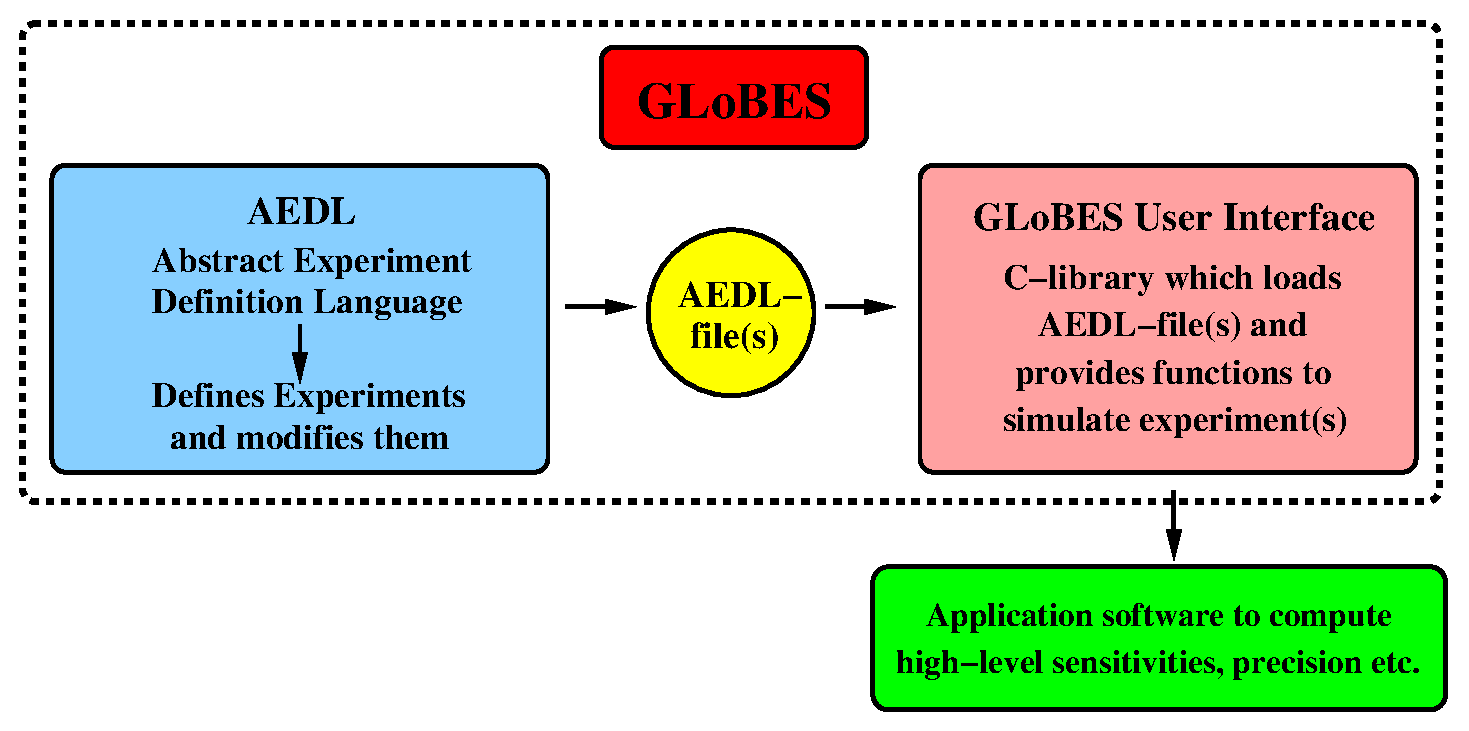
\includegraphics[width=14cm]{GLOBES}
\end{center}
\caption{\label{fig:GLOBES} General concept of the \GLOBES\ package.}
\end{figure}

\GLOBES\ allows to simulate experiments with stationary neutrino point 
sources, where each experiment is assumed to have only one neutrino source.
Such experiments are neutrino beam experiments and reactor experiments. 
Geometrical effects of a continuous source distribution, such as in the sun or the 
atmosphere, can not be described. In addition, sources with a physically 
significant time dependencies can not be studied, such as  supernov\ae. 
However, in \GLOBES\ 3.0 and higher, new flexibility is introduced by the
concept of user-defined systematics. This new feature allows the cross-definition
of systematical errors over different experiments. In principle, 
this mechanism can be used for the combination of several discrete sources
and one detector, or several detectors and one source, or several sources and
several detectors. In addition, already implemented
concepts of \GLOBES\ have been used for indirect simulations of geometrical
effects. For example, the mapping of the detector location on the neutrino
energy has been simulated in \Ref~\cite{Rolinec:2006xr} by the use of
variable bin widths.

On the experiment definition side, either built-in neutrino fluxes
(\eg, neutrino factory, beta beam) or arbitrary, user-defined fluxes can be used. 
Similarly,
arbitrary cross sections, energy dependent efficiencies,
energy resolution functions as well as the considered oscillation channels, 
backgrounds, and many other properties can be specified. 
For the systematics, energy
normalization and calibration errors can be simulated, or the
systematics can be completely user-defined. Note that
energy ranges and windows and bin widths can be
(almost) arbitrarily chosen, including bins of different
widths. Together with \GLOBES\ comes a number of
pre-defined experiments in order to demonstrate the capabilities
of \GLOBES\ and to provide prototypes for new experiments.
In addition, they can be used to test new physics ideas with
complete experiment simulations.
% Examples for these prototypes are the \MINOS , \ICARUS , and
% \OPERA\ simulations from \Ref~\cite{Huber:2004ug}, the
% \JHFSK\ and \NUMI\ superbeam simulations from \Refs~\cite{Huber:2002mx,
% Huber:2002rs}, the \JHFHK\ superbeam upgrade simulation from
% \Ref~\cite{Huber:2002mx}, the neutrino factory simulations from
% \Ref~\cite{Huber:2002mx}, and the reactor experiment simulations from
% \Ref~\cite{Huber:2003pm}. Other projects using earlier versions
% of the \GLOBES\ software include \Refs~\cite{Huber:2003ak,Ohlsson:2003ip,Winter:2003ye,Antusch:2004yx}.

With the C-library, one can extract the $\Delta \chi^2$ for all defined 
oscillation channels for an experiment or any combination of experiments.
Of course, also low-level information, such as oscillation
probabilities or event rates, can be obtained. \GLOBES\ includes the
simulation of neutrino oscillations in matter with arbitrary matter 
density profiles. In addition, it allows to simulate the matter density
uncertainty (see, \eg, \Refs~\cite{Huber:2002mx,Ohlsson:2003ip}) and to 
extract the precision on the matter density (see, \eg, \Refs~\cite{Winter:2005we,Gandhi:2006gu}).
 As one of the most
advanced features of \GLOBES , it provides the technology to 
project the $\Delta \chi^2$, which is a function of all oscillation
parameters, onto any subspace of parameters by local minimization. 
This approach allows the inclusion of multi-parameter-correlations,
where external constraints (\eg, on the solar parameters) can be imposed, too.
Applications of the projection mechanism include the projections onto 
the $\stheta$-axis and the $\stheta$-$\deltacp$-plane. In addition, 
all oscillation parameters can be kept free to precisely localize 
degenerate solutions.

\section{User-defined systematics and changes in the systematics implementation}

How defined, what good for (physics examples: T2KK, Reactor-paper,).
Compare to standard systematics (nuisance parameters)

\section{User-defined priors}

How defined, what good for (physics examples: AstroNus, Schwetz priors, atm. neutrinos, octant degeneracy,
).

\section{Simulation of non-standard physics with GLoBES}

Eg. Damping, Hamiltonian, MAVANS, Toshi etc.

\section{Simulation of new experiment features and \AEDL\ changes}

\bi
\item 
 Built-in $\beta$-beam fluxes
\item
 New AEDL features
\item
 New AEDL files in standard GLoBES delivery + changes to existing ones
\ei

Beta beams paper!

\section{New platform and interpreter support, new ways to improve the performance}

\bi
\item
 PERL?
\item 
 Windows?
\item
 Better RedHat support
\item
 Changes in installation scheme
\ei


\bi
\item 
 GLoBES on clusters, Condor; parallized code; static links
\item 
 64 bit support
\item 
 New minimization algorithm!?
\ei

Sophisticated \GLOBES\ simulations with several experiments and complicated
parameter correlations can take several days to finish even on modern computers.
To mitigate this problem as far as possible, we have taken several steps to
optimize the performance of the multi-dimensional minimizations, which are at
the heart of each \GLOBES\ $\chi^2$ analysis.

Firstly, the \GLOBES\ minimizers distinguish between minimization over
oscillation parameters and minimization over systematics parameters.
This is necessary because each step in the oscillation parameter space
requires a time-consuming re-computation of oscillation probabilities,
while a modification of the systematics parameters does not. The standard
procedure is to perform a full minimization in systematics space after each
step in oscillation space. This avoids interference of the two categories
of parameters, and is known to have excellent convergence properties.
The numerical method that does the minimization is the Powell
algorithm~\cite{Press:NumRecip}.

In \GLOBES\ 3.0, we provide an alternative method, which does the full minimization
in one go and is therefore several times faster in most cases. In this algorithm,
each Powell iteration over oscillation parameters is followed by one iteration
over systematics parameters. Since there may be some pathological cases where this
interleaved minimization strategy behaves differently than the old method,
it is by default not used in \GLOBES\ 3.0. This ensures maximal compatibility
with old application programs, but it requires users who wish to benefit from the
new algorithm to explicitly select it by an API function call.

Besides optimizing the minimization functions, it is also mandatory to
optimize the routines which are called by them to calculate $\chi^2$
for one specific set of parameters. In particular, the computation of
oscillation probabilities, which has to be done every time the oscillation
parameters have changed, should be as efficient as possible. The most expensive
step here is the diagonalization of the hermitian $3\times3$ neutrino Hamilton
operator in matter. The LAPACK rotuines~\cite{Anderson:LAPACK}, which were
used to solve this eigenproblem in previous versions of \GLOBES, turned out
not to be the optimal choice because they are mainly optimized for very large
matrices~\cite{Kopp:2006wp}. In the case of the small and usually well-conditioned
matrices appearing in \GLOBES, they spend too much time evaluating their parameter
list and planning the optimal diagonalization strategy. Therefore, \GLOBES\ now
relies an algorithm which has been designed specifically for the diagonalization
of hermitian $3\times3$ matrices. It is essentially the extremely fast analytical
algorithm discussed in~\cite{Kopp:2006wp}, but for the rare cases where this may become
inaccurate, it falls back to the QL method from~\cite{Press:NumRecip}.



\section{Summary and conclusions}


\subsection*{Acknowledgments}

For the current version of \GLOBES , we would like to 
thank Thomas Schwetz, who has been pushing the software to the edge in the 
past few years. Furthermore, we would like to thank Tommy Ohlsson,
Toshihiko Ota, and Julian Skrotzki for using and testing unpublished new features of the software.
%
The development of \GLOBES\ is currently being supported by the Studienstiftung des Deutschen Volkes [JK] and the
 Emmy Noether-Program of Deutsche Forschungsgemeinschaft [WW].
%
In the past, the following institutions and organizations have supported 
members of the \GLOBES\ team: Technische Universit\"at M\"unchen,
Max-Planck-Institut f\"ur Physik, SFB 375 for astro-particle physics
of Deutsche Forschungsgemeinschaft, Studienstiftung des Deutschen Volkes,
Institute for Advanced Study, Princeton, W. M. Keck Foundation, and National Science Foundation.

\bibliographystyle{apsrev}
\bibliography{references}

\end{document}

